\subsection{FreeRTOS}

Στην εισαγωγή αναφέραμε τον κύκλο ζωής εντολών, τον τρόπο
που συνήθως ο επεξεργαστής εκτελεί instructions. Η ιδέα
αυτή της ψευδαίσθησης του παραλληλισμού είναι αρκετά σύνηθες
σε εφαρμογές λειτουργικών συστημάτων. Το FreeRTOS, συγκεκριμένα
η υλοποίηση του ESP-IDF, δεν διαφέρει καθόλου.

Πρόκειται για ένα όσο το δυνατόν πιο μινιμαλιστικό λειτουργικού
σύστημα. Αποτελείτε απλώς από:

\begin{enumerate}
  \item Έναν scheduler.
  \item Tasks που τρέχουν με βάση τον scheduler.
  \item Hooks που τρέχουν όταν παίρνουν μέρος events του λειτουργικού συστήματος.
  \item Αντικείμενα που επιτρέπουν την επικοινωνία μεταξύ
    tasks.
\end{enumerate}

Υποστηρίζονται πολλοί scheduling αλγόριθμοι αλλά αναφερόμαστε κυρίως
στο default που χρησιμοποιεί το ESP-IDF. Ο default scheduler είναι
κατά κύριο λόγο προεκτοπιστικός (preemptive) το οποίο σημαίνει ότι μια
διεργασία μπορεί να διακοπεί οποιαδήποτε στιγμή από κάποια άλλη
υψηλότερης ή ίσης προτεραιότητας. Κάθε task έχει σταθερή προτεραιότητα
(fixed priority). Όταν δύο tasks έχουν ίση προτεραιότητα χρησιμοποιούνται
time slices για να αλλάξει η κατάσταση τους.

Όπως φαίνεται στο σχήμα \ref{fig:task_states} τα tasks έχουν 4 καταστάσεις:

\begin{enumerate}
\item Ready, μπορούν να καλεστούν για να τρέξουν.
\item Running, τρέχουν αυτήν την χρονική στιγμή.
\item Blocked, δεν τρέχουν αυτήν την χρονική στιγμή.
\item Suspended, το task δεν είναι διαθέσιμο στον scheduler.
\end{enumerate}
    
\begin{figure}[!htb]
    \centering
    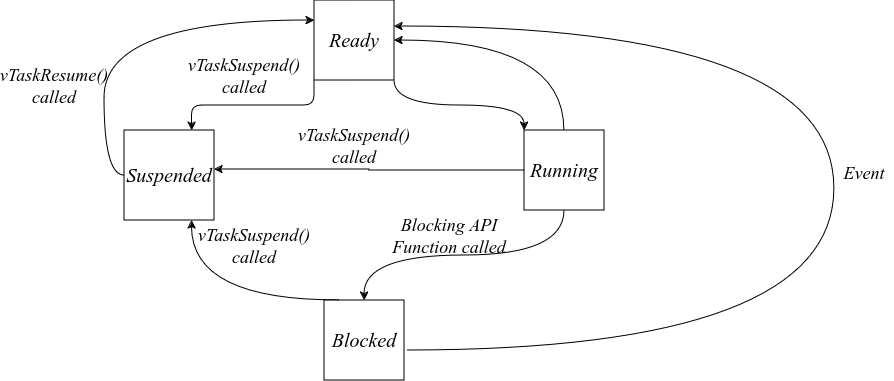
\includegraphics[scale=0.4]{images/espidf/freertos_tasks.png}
    \caption{Καταστάσεις διεργασιών}
    \label{fig:task_states}
\end{figure}

Τα states \verb|Ready| και \verb|Running| αλλάζουν συνεχώς ανάλογα
με τις προτεραιότητες και τα ενδιάμεσα blocks. Όσο αναφορά το \verb|Suspended|
state σπάνια το διαχειριζόμαστε άμεσα σαν χρήστες και κατά κύριο λόγο καλείτε
όταν κάνουμε \verb|vTaskDelete(NULL)| για να "σβήσουμε" το task που τρέχει
αυτήν την στιγμή.

Για να δημιουργήσουμε ένα task που ο scheduler μπορεί να δει χρησιμοποιούμε:

\begin{lstlisting}[language=C]
BaseType_t xTaskCreate(TaskFunction_t pvTaskCode,
                         const char * const pcName,
                         const configSTACK_DEPTH_TYPE uxStackDepth,
                         void *pvParameters,
                         UBaseType_t uxPriority,
                         TaskHandle_t *pxCreatedTask
                       );
\end{lstlisting}

Η συνάρτηση φαίνεται πολύ πιο περίπλοκη από ότι είναι την πραγματικότητα:

\begin{enumerate}
\item Το \verb|TaskFunction_t| είναι απλώς ένας δείκτης σε μια συνάρτηση που
  επιστρέφει \verb|void| και έχει \verb|void*| ως παράμετρο. Αυτή η συνάρτηση είναι
  ο κώδικας του task που θέτει ο χρήστης.
\item Το \verb|const char* const| είναι προφανές, δεν έχει ιδιαίτερη χρησιμότητα και
  υπάρχει κυρίως για λόγους debugging.
\item Το \verb|const configSTACK_DEPTH_TYPE uxStackDepth| είναι το
μέγεθος του stack σε words (όχι bytes). Κάθε task έχει ξεχωριστό stack
και ο χρήστης είναι υπεύθυνος να προβλέψει το πιο είναι το ελάχιστο
απαραίτητο μέγεθος για λόγους βελτιστοποίησης.
\item Το \verb|void*| είναι οι παράμετροι που το task δέχεται. Δεν μπορούμε
  να προσθέσουμε stack-based values εδώ επειδή κάποια στιγμή θα βγούνε από το
  scope και θα καταλήξουμε σε ένα null pointer dereference error. Προφανώς
  αυτό ισχύει σε οποιαδήποτε τιμή που δείχνει σε μη προσβάσιμη μνήμη.
\item Το \verb|UBaseType_t| είναι ένα \verb|unsigned int| που αντιπροσωπεύει την προτεραιότητα.
\item Το \verb|TaskHandle_t| είναι προαιρετικό αλλά επίσης χρήσιμο για debugging,
  είναι ένα \verb|typedef| ενός δείκτη οπότε αν δεν θέλουμε να το ορίσουμε το θέτουμε
  ως \verb|NULL|.
\end{enumerate}
